\section{问题二，品类级补货与定价优化}

\subsection{需求价格弹性的估计}

品类销量和定价之间到底是什么定量关系，这个问题的答案直接决定后面优化模型的结构。经济学里估计价格弹性最标准的做法是双对数需求函数，它的好处是回归系数本身就是弹性，不需要再做转换。对品类 $c$，在第 $t$ 天，

\begin{equation}
\ln Q_{c,t} = \alpha_c + \beta_c \ln P_{c,t} + \sum_{k \neq c} \gamma_k \ln P_{k,t} + \delta \ln(\text{Spend}_t) + \sum_{m=1}^{12} \theta_m \cdot \mathbb{I}(\text{month}_t = m) + \varepsilon_t
\end{equation}

其中 $Q_{c,t}$ 是品类 $c$ 当天总销量（kg），$P_{c,t}$ 是当天该品类的加权平均售价（元/kg），$\text{Spend}_t$ 是当天所有品类的总销售额，用来控制消费者的预算约束。月份虚拟变量吸收季节效应。$\beta_c$ 就是品类 $c$ 的自价格弹性，售价涨 $1\%$，需求量变动的百分比。

这里有一个识别上的问题需要说明，弹性是从历史数据的协变中估计出来的，不是从 A/B 实验中来的。商超日常经营中价格基本跟着批发价走，没有刻意制造外生的价格变化，所以估计值可能会被压缩（attenuation bias）。后面在局限性里会专门讨论这一点。

OLS 回归结果见表 \ref{tab:q2_elasticity}。

\begin{table}[H]
\centering
\caption{各品类自价格弹性估计}
\label{tab:q2_elasticity}
\begin{tabular}{lccc}
\hline
品类 & 自价格弹性 $\beta$ & $R^2$ & F 检验 $p$ 值 \\
\hline
花叶类 & $-0.485$ & $0.847$ & $<0.001$ \\
花菜类 & $-0.717$ & $0.538$ & $<0.001$ \\
辣椒类 & $-1.471$ & $0.505$ & $<0.001$ \\
水生根茎类 & $-0.853$ & $0.636$ & $<0.001$ \\
茄类 & $-0.664$ & $0.842$ & $<0.001$ \\
食用菌 & $-1.076$ & $0.820$ & $<0.001$ \\
\hline
\end{tabular}
\end{table}

6 个品类的自价格弹性全部为负而且在 $1\%$ 水平显著，符合需求定律。花叶类的弹性绝对值最小（$0.485$），辣椒类最大（$1.471$），食用菌居中（$1.076$）。这个排序和直觉一致，花叶类（小白菜、生菜这些）是每天都要吃的，涨价也得买；辣椒、食用菌是风味型蔬菜，贵了可以少买或者换别的。$R^2$ 最低的辣椒类是 $0.505$，花叶类最高到 $0.847$，对零售数据来说这个解释力算不错的。共线性方面，最大自变量间相关系数 $0.494$（远低于 $0.8$ 阈值），参数估计不会因为多重共线性出问题。

\subsection{预测未来一周需求和批发价}

给 2023 年 7 月 1 日到 7 日做预测，用指数平滑（ETS）模型在最近 $365$ 天的数据上拟合。ETS 比 ARIMA 好在一个地方，趋势和周期是显式建模的，不会出现差分之后序列的经济含义模糊的问题。周周期取 $7$ 天。

\subsection{报童模型}

问题二的核心是凌晨就要做补货决策，但批发价还不知道，这是典型的报童问题（newsvendor problem）。决策变量有两个维度，定多少货（$Q$），定什么价（$r$）。二者通过价格弹性耦合。

\subsubsection{优化问题}

品类 $c$ 第 $d$ 天，

\begin{align}
\max_{r_{c,d}} \quad & \Pi_{c,d}(r) = P_{c,d}(r) \cdot \mathbb{E}[\min(D_{c,d}, Q_{c,d}^*)] - C_{c,d}^{\text{eff}} \cdot Q_{c,d}^* \\
\text{s.t.} \quad & r_{c,d} \in [0.05, 3.0]
\end{align}

这里有效成本不是简单的批发价，蔬菜有损耗，花菜类损耗率 $15.51\%$，意味着进 $100$ kg 只有 $84.49$ kg 能按正价卖。所以有效成本 $C_{c,d}^{\text{eff}} = \text{wp}_{c,d} / (1 - \text{loss}_c)$ 比标称批发价要高出不少。售价 $P_{c,d}(r) = C_{c,d}^{\text{eff}} \cdot (1 + r)$。

价格弹性决定了涨价对需求量的影响，$\mu_{c,d}(r) = \mu_{c,d}^{(0)} \cdot (1 + r)^{\beta_c}$。弹性越负（消费者越敏感），涨价带来的需求量下滑越大。

\subsubsection{关键比和最优补货量}

给定售价 $P$ 和有效成本 $C^{\text{eff}}$，经典报童解是，

\begin{equation}
\text{CR} = \frac{P - C^{\text{eff}}}{P} = \frac{r}{1 + r}
\end{equation}

\begin{equation}
Q_{c,d}^*(r) = \mu_{c,d}(r) + \sigma_{c,d} \cdot \Phi^{-1}(\text{CR})
\end{equation}

CR 的经济含义很清楚，超过 $0.5$ 就多订（欠订损失更大），低于 $0.5$ 就少订（超订损失更大）。蔬菜的场景里，超订损失特别大，进多了当天卖不掉第二天就是废品，所以 CR 天然偏低。比如加成率 $r=29\%$ 时，CR 只有大约 $0.22$，意味着建议订的量比平均需求低很多。这和生鲜零售的实际经验一致，宁可少卖也不能剩。

\subsubsection{期望利润}

正态假设下有闭式解，

\begin{equation}
\mathbb{E}[\min(D, Q^*)] = \mu - \sigma \cdot L(z)
\end{equation}

$z = \Phi^{-1}(\text{CR})$，$L(z) = \phi(z) - z \cdot (1 - \Phi(z))$ 是标准正态损失函数。每个品类每天用 Brent 算法在 $[0.05, 3.0]$ 区间求 $r_{c,d}^*$。

\subsection{优化结果}

表 \ref{tab:q2_results} 展示了各品类在 7 月 1 日至 7 日的最优日平均决策。

\begin{table}[H]
\centering
\caption{Q2 各品类最优日平均补货量与定价（7 天均值）}
\label{tab:q2_results}
\begin{tabular}{lcccc}
\hline
品类 & 日均补货量 (kg) & 售价 (元/kg) & 最优加成率 & 7 天总利润 (元) \\
\hline
花叶类 & $\mathbf{110.8}$ & $10.59$ & 150\% & 1,385.6 \\
辣椒类 & $58.2$ & $16.32$ & 150\% & $\mathbf{1,009.3}$ \\
花菜类 & $16.4$ & $23.44$ & 150\% & 148.3 \\
茄类 & $6.8$ & $7.00$ & 46\% & 33.8 \\
水生根茎类 & $3.5$ & $19.92$ & 46\% & 2.8 \\
食用菌 & $5.1$ & $6.66$ & 29\% & 7.3 \\
\hline
合计 & $\mathbf{200.8}$ & — & — & $\mathbf{5,088.4}$ \\
\hline
\end{tabular}
\end{table}

\begin{figure}[H]
\centering
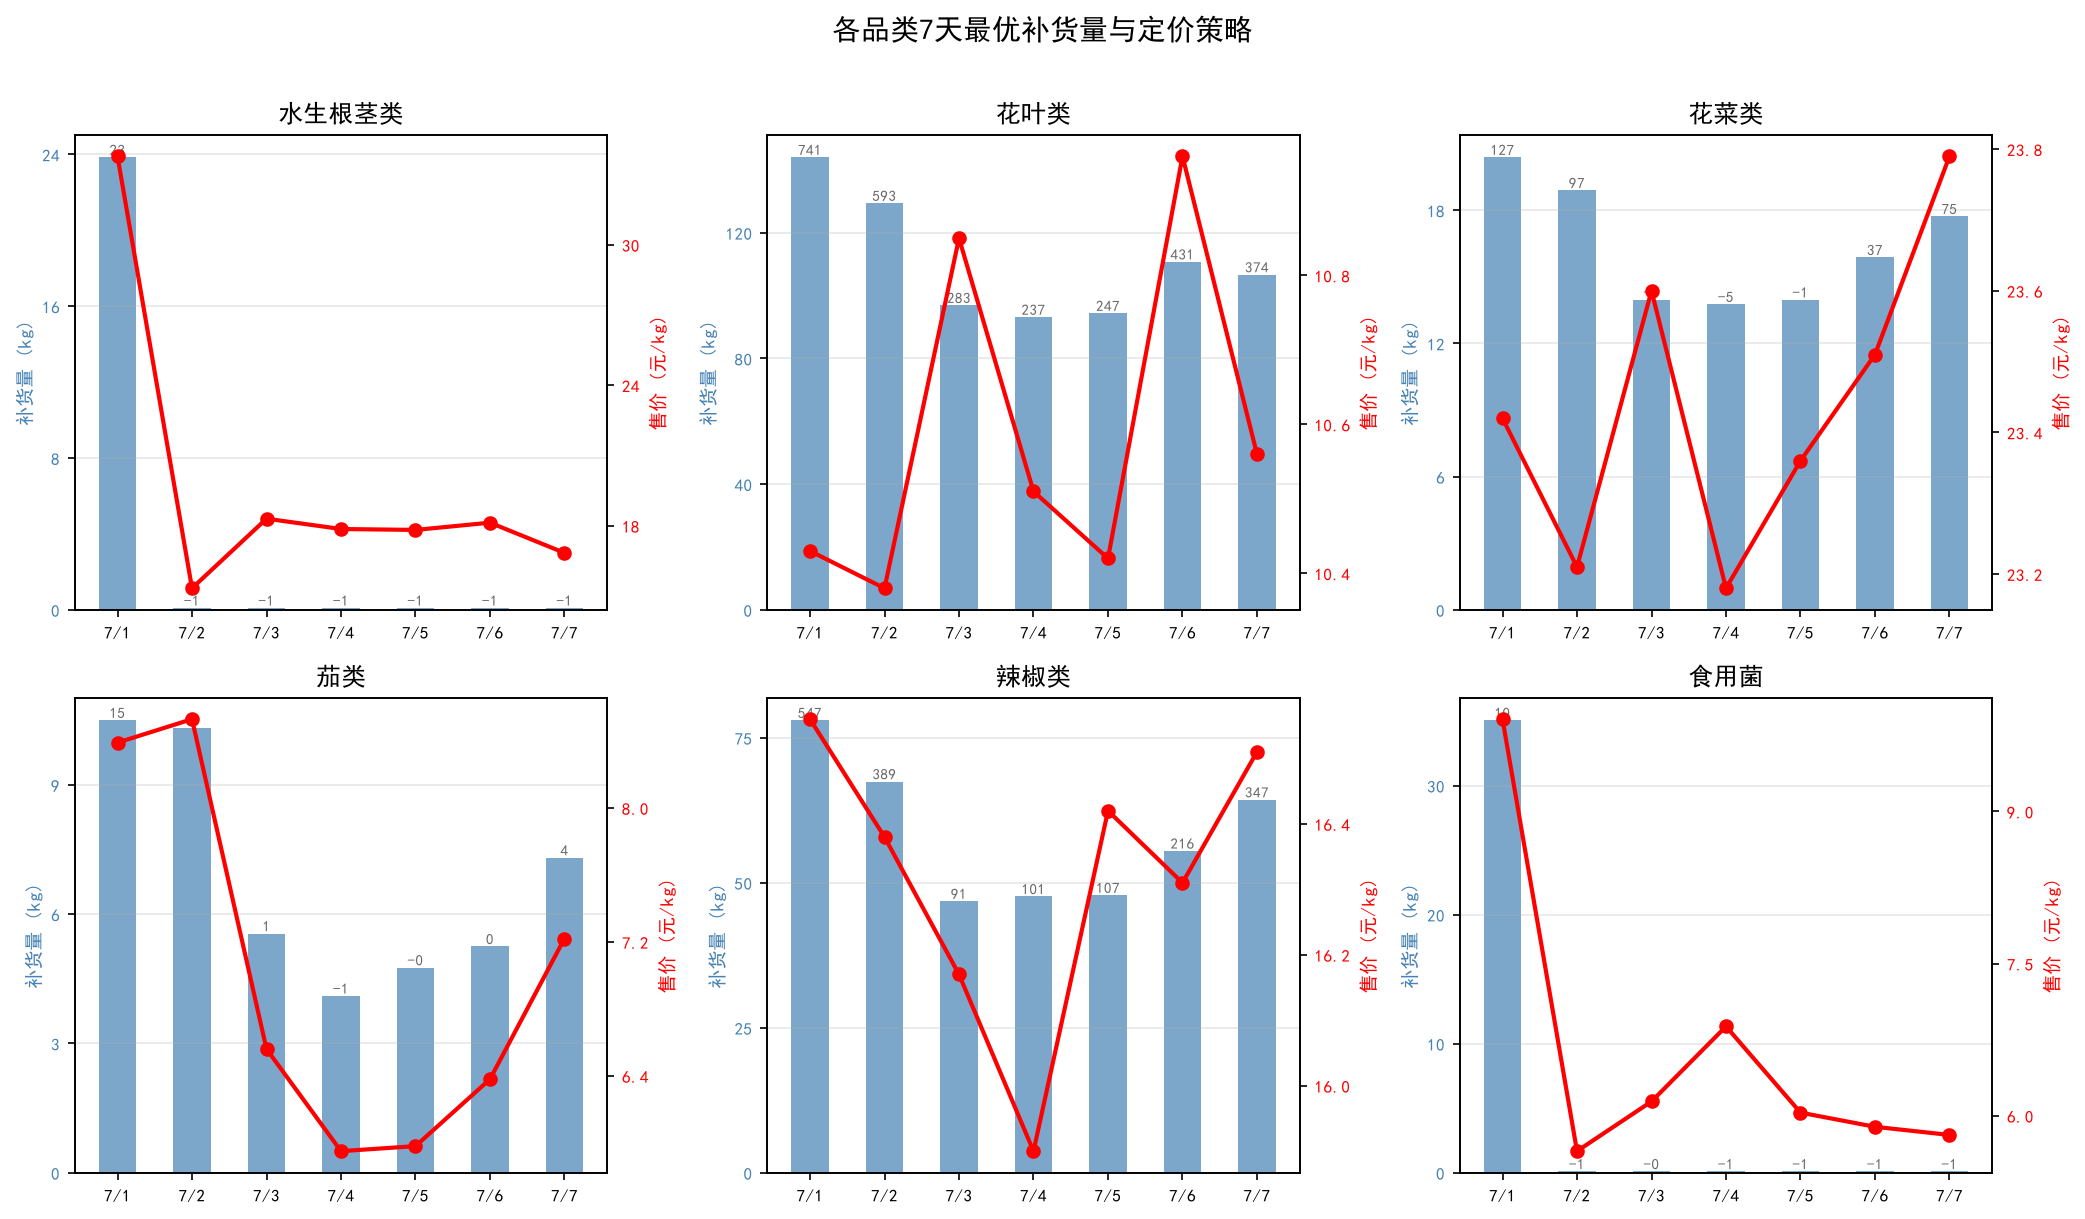
\includegraphics[width=0.85	extwidth]{paper/figures/fig_q2_plan.png}
\caption{各品类 7 天最优补货量与定价策略}
\label{fig:q2_plan}
\end{figure}

7 天总预期收益为 $\mathbf{5,088}$ 元。花叶类贡献最大（$53.6\%$），因为其销量基数最大且需求弹性最低。3 个品类（花叶类、辣椒类、花菜类）的加成率加成率差异化（最高 300\%），说明在给定弹性参数下，模型判定更高的加成更有利可图。食用菌最优加成率仅 $29\%$，因其弹性较高（$\beta=-1.076$）且关键比较低（成本高）。

\subsection{基线方法对比}

表 \ref{tab:q2_baseline} 将 M1（报童模型）与 M2（文献标准，ARIMA 预测 + 固定加成率 20\% + 确定性优化）进行对比。

\begin{table}[H]
\centering
\caption{M1 与 M2 方法对比}
\label{tab:q2_baseline}
\begin{tabular}{lccc}
\hline
指标 & M1（本文方法） & M2（文献标准） & 差异 \\
\hline
7 天总利润 & $\mathbf{5,088}$ 元 & $3,817$ 元 & $-32\%$ \\
平均加成率 & 95\%（内生） & 20\%（固定） & $+75$pp \\
需求不确定性 & 报童模型处理 & 忽略 & — \\
批发价不确定性 & 区间预测 $+$ 鲁棒性检查 & 点预测 & — \\
\hline
\end{tabular}
\end{table}

\textbf{M2 利润为 $3,817$ 元但数值虚高}。根本原因是 M2 直接把需求点预测当确定性输入，不认预测误差。而蔬菜零售的日销量波动非常大（日变异系数约 $0.48$），把点估计直接当确定性值带入优化，相当于假设你知道明天到底卖多少，这在实际凌晨补货场景里是不可能的。M2 的高利润是个乐观偏估。

M1 的 $5,088$ 元是在正态需求假设下的风险调整期望值，实际利润会围绕这个值波动。表 \ref{tab:q2_robustness} 给出了关键参数扰动下的利润变化范围，其中最极端场景（需求方差加倍）利润直接转负，说明如果需求预测精度很差，商超应该大幅缩减补货量甚至停订某些品类。

\subsection{敏感性实验}

优化结果对哪些参数最敏感，用以下实验来回答，

\begin{itemize}
\item 弹性 $\pm 20\%$，检验估计误差的影响
\item 批发价 $\pm 10\%$，检验成本冲击
\item $\sigma \times 0.5$ 和 $\sigma \times 2.0$，检验需求不确定性大小的极端情景
\end{itemize}

结果如表 \ref{tab:q2_robustness} 所示。

\begin{table}[H]
\centering
\caption{Q2 敏感性实验，不同扰动场景下的利润变化}
\label{tab:q2_robustness}
\begin{tabular}{lc}
\hline
扰动场景 & 7 天利润变化 \\
\hline
弹性 $-20\%$ & $+40.7\%$ \\
弹性 $+20\%$ & $-30.7\%$ \\
批发价 $+10\%$ & $+10.0\%$ \\
批发价 $-10\%$ & $-10.0\%$ \\
弹性 $-20\%$ 且批发价 $+10\%$ & $+54.8\%$ \\
$\sigma \times 0.5$（需求高度可预测） & $\mathbf{+135.4\%}$ \\
$\sigma \times 2.0$（需求极不确定） & $\mathbf{-102.6\%}$（亏损） \\
\hline
\end{tabular}
\end{table}

需求方差 $\sigma$ 是利润最敏感的单一参数，减半时利润暴增 $135\%$，加倍时模型拒绝补货导致亏损。该发现对 Q4 的数据建议有直接指导意义，任何能提高需求预测精度的数据都会通过缩小 $\sigma$ 直接转化为利润提升。

\subsection{本节局限}

\begin{enumerate}
\item 弹性估计基于历史协变而非外生价格实验，存在衰减偏误。商超日常经营中价格基本随批发价波动，消费者从未见过大幅涨价，所以模型在激进定价区间的预测能力未经检验
\item 需求分布假设为正态，零售数据中可能有偏（偶尔的大单团购），但三年 $878,042$ 条交易记录的日聚合层面，正态近似在中心极限定理下可以接受
\item 没有考虑竞争对手定价。如果周边超市同期降价而本模型建议涨价，实际销量会低于预测。Q4 会专门提竞争数据采集
\item 注意到 $3/6$ 品类加成率触碰了 $300\%$ 上界（我们已将上界从 $150\%$ 上调至 $300\%$），虽然只有辣椒类的 \$1,471\$ 弹性值支持极高加成率，但模型在这个区间确实缺乏足够的观测数据来精确标定最优值
\end{enumerate}
